\documentclass[12pt,a4paper]{article}
\usepackage[latin1]{inputenc}

\usepackage{amsmath}
\usepackage{amsfonts}
\usepackage{amssymb}
\usepackage{graphicx}
\usepackage{natbib}
\usepackage{setspace}
%\doublespacing


%\title{Simulating the initial conditions of star formation and the influence of the environment.}


\begin{document}

\author{PI: Mordecai-Mark Mac Low, American Museum of Natural History, New York}
\title{Simulating the formation of star-forming regions in a galactic environment.}


\section{Introduction}

In this proposal we request allocation to pursue a series of numerical simulations addressing a number of open questions about the formation, the dynamics and the evolution of star-forming regions in a galactic disk environment.
The simulations proposed here include several physical processes such as, supernova (SN) feedback, magnetic fields, galactic gravitational potential, gas self-gravity, parametrized gas cooling and photoelectric heating. 
The proposed simulations cover 6 orders of magnitude in spatial scales and temperature range and more than 7 orders of magnitude in densities, essential for the study of star-formation. 
Our primary goals include:

\begin{itemize}

	\item We will focus on the formation and evolution of self-gravitating structures in a turbulent, magnetized interstellar medium (ISM) near the galactic midplane; we will do so by capturing the vertical stratification of the ISM in the galaxy with our elongated box. 
	We then concentrate our analysis to the regions around the midplane, $|z| < 50 \, pc$ where most of the cold gas lives, and follow the assembly of self-gravitating structures and their evolution for several $Myr$. 
	These simulations are critical for understanding the formation rate and lifetime of self-gravitating structures in the galaxy.
	
	\item We will study the development of the initial conditions for star formation in a collapsing cloud; Focusing resolution (localized mesh-refinement) on self-gravitating clouds, we will follow the evolution of the cloud while it fragments and collapses, paying special attention to the the importance of filamentary structures in the star-formation process. 
	We will concentrate in the dynamics of the gas in, and near the filament and effects of the magnetic fields in the thickness, orientation and fragmentation of filaments. 
	This simulations will be critical for understanding the influence of the geometry and the initial conditions in the star formation process.
	
\end{itemize}

This proposal will constitute the main allocation for the completion of the PhD thesis of co-I Juan Iba\~nez-Mejia, working under the supervision of PI Mordecai-Mark Mac Low. 
These project is supported by the NSF and is part of a joint collaboration of mixed researchers with US and German affiliations.



\section{Star Formation in Galactic Disks}
	
All of the observed star formation occurs in galaxies or protogalaxies. 
A correlation between stellar birth and large-scale dynamics has been observed in star-forming galaxies. 
Understanding what controls the star formation rate in the galaxy is crucial for understanding galaxy evolution.  
There are still a number of open questions about the control and the details of the star formation process in the galaxy, we list two that we will address with the simulations proposed here:

\begin{itemize}

	\item[1] \textbf{Formation and lifetime of molecular clouds: }

		Stars form in the dense, self gravitating gas that efficiently cools down and collapses under it's own self gravity. 
		The formation of these clouds is triggered by converging flows, gravitational instability and fragmentation.
		Resistance to collapse, on small scales, comes from magnetic and thermal pressure, and random turbulent motions triggered from supernova, radiation and wind feedback from stars.
		It is still unknown what effect might the environment play in the lifetime and star formation efficiency of star forming clouds.
			
	\item[2] \textbf{The initial conditions for star formation: }

		Star formation occurs in a clustered fashion within turbulent, dense molecular clouds.
		Turbulence creates a hierarchy of clumps which begin contracting as turbulence decays.
		While dense region contract, individual clumps collapse to form stars, and in clustered regions, clumps may merge while collapsing.
		Finally, feedback terminates the star formation dissipating the parent cloud.
		The amount of interaction and efficiency of stellar feedback in the cloud dissipation strongly depends on the yet unknown initial conditions.

		%\item[3] \textbf{What is the }
		%	Dont remember correctly what I wanted to put here.


\end{itemize}

We propose to study the process of molecular cloud assembly, evolution and collapse in an active turbulent medium. 
The simultaneous action of supersonic turbulence, self-gravity, magnetic fields, photoelectric heating, gas cooling, midplane pressure and the galactic fountain provide a unique combination of some of the most important physical processes involved in the star formation in the galaxy.
Furthermore, the localized zoom-in capabilities enable us to resolve the turbulent cascade down to very small scales, resolving individual star forming sites.


\subsection{Stratified box model}

In order to gain a complete picture of the turbulent energetics in galactic disks, we must resolve the dynamics from a wide range of scales $10^{4} > l > 10^{-3} \, pc$ and incorporate the most important physics and thermodynamics over the complete range of temperatures $10 < T < 10^{8} \, K$ and densities $10^{-5} < n < 10^{2} cm^{-3}$.
We will extend the work of \citet{JoungMacLow2006,Joung2009, Hill2012}, simulating a vertical column of the magnetized ISM with turbulence driven by SN explosions.                            
	                                                                                                                                                                                    
To simultaneously resolve the expansion of hundreds-pc-size million degree super bubble gas, we require a minimum resolution of $\sim 2 pc$ near the midplane, for the subpc-size condensation and collapse of cold ($T \sim 20 \, K$) clouds, a minimum resolution of $\sim 10^{-2} pc$ in the collapsing structures is implemented and to trace the kpc-size Galaxy fountain flow of gas out of the midplane into the halo and back the vertical length of the box extends to $z \pm 20 \, kpc$ \citep{Avillez&Breitschwerdt2004, Joung2012, Hill2012}.
	
Previous models of the SN driven turbulent box lacked the action of self-gravity and suffered from low resolution on the dense gas \citet{JoungMacLow2006,Joung2009, Hill2012}, so they could not follow gravitational collapse and directly measure the star formation rate.
	
We include the action of gas self-gravity in this work to directly follow the formation and collapse of self gravitating structures in a turbulent ISM using the optimized multigrid Poisson solver \cite{Daley2012}.
Gravitational collapse leads to runaway collapse that can not be numerically resolved, therefore we will also include the formation of sink particles \citep{Bate95, Federrath2010}, to replace unresolved gravitational collapse by stellar sink particles.
This allow us to understand how quickly gravitational collapse sets in after molecular cloud formation and the resulting characteristics of the stellar clusters formed inside the cloud and compare them to the idealized simulations of isolated molecular clouds \citep{Dale2014, Girichidis2011, Bate2009}.

\begin{figure}
	\includegraphics[scale=0.32]{Figures/Midplane_Before_5MyAfter-SG.eps} 	
	% include the self gravitating figure.
	\caption{column density plot along the vertical direction before and after the action of self-gravity.}
	\label{midplane_nosg_sg}
\end{figure}
	
Gas self gravity greatly influences the gas dynamics and the morphology of the midplane compared to the turbulence-only simulations.
Figure \ref{midplane_nosg_sg}, shows a column density plot perpendicular to the galactic midplane computed with this year's allocation.
The collapse of structure along the shortest direction is appreciated with the formation of a complex network of coherent filaments in the midplane.
This filaments are swept together by global gravitational collapse, growing in mass as they accrete from their environment and merge with each other.
While the mass and the filament density steadily grow during collapse, the filament turns unstable and fragmentation sets in forming clumps, the ideal candidates for cluster formation sites.
	
With the inclusion of self-gravity we will measure the total amount of collapsing gas and the resulting star formation rate in the box.
We will then compare it with the star formation rate required to maintain the input SN rate, which will provide critical knowledge for understanding if star formation is primarily determined by the local physics of cooling and cloud formation in a non-rotating disk.
	
Despite the number of physical processes already accounted in this model, we will not yet be able to understand the self-regulation mechanism of star formation.
There are still a number of missing physical processes required to understand the complete cycle of stars, such as self-consistent stellar feedback. 
Some of these missing physical processes are being currently developed and will be included in the model shortly. 

Stellar feedback is suggested to play a crucial role in cloud formation and destruction (citations). 
To investigate the efficiency of radiative stellar feedback in quenching the star formation, we will implement a radiative transport model using stellar sink particles as sources of radiation and implement the adaptive ray tracing technique developed by \citet{Wise&Abel2011}.
	
Stellar sink particles are not only sources of radiation but energetic stellar winds ejected from their surface. 
A wind feedback model implementation requires knowledge of the mass ejection rate and wind velocity given the stellar mass and age.
This parameters are computed from the latest set of the Geneva group stellar evolution tracks \citet{Ekstrom2012, Georgy2012, Georgy2013}.

Finally, massive stars live quick and die young and end their lives in massive SN explosions.
We already have a prescription for SN explosions which will be correlated with sink particles.
	
\subsection{Zoom-in models}
	
We will perform zoom-in simulations applying localized extra mesh refinement on the jeans unstable gas to specific, gravitationally bound clouds in the simulated volume.
The increased resolution will allow us to directly observe the formation and the dynamics of gravitationally bound molecular clouds with sub-pc resolution providing cloud morphologies, turbulent, density and magnetic structures and cloud lifetimes.
	
We will identify interesting structures in our canonical runs (see figure \ref{midplane_nosg_sg}), then specify a refinement region to follow them allowing many more levels of refinement within it.
Because the timestep drops in the zoom-in region, this is primarily useful for following individual dense structures, while the rest of the simulation acts as an evolving boundary condition for the region.
This is more realistic than the usual practice of treating giant molecular clouds as isolated, evolving objects \citep{Dale2014, Girichidis2011, Bate2009}
	
\begin{figure}
	\centering
	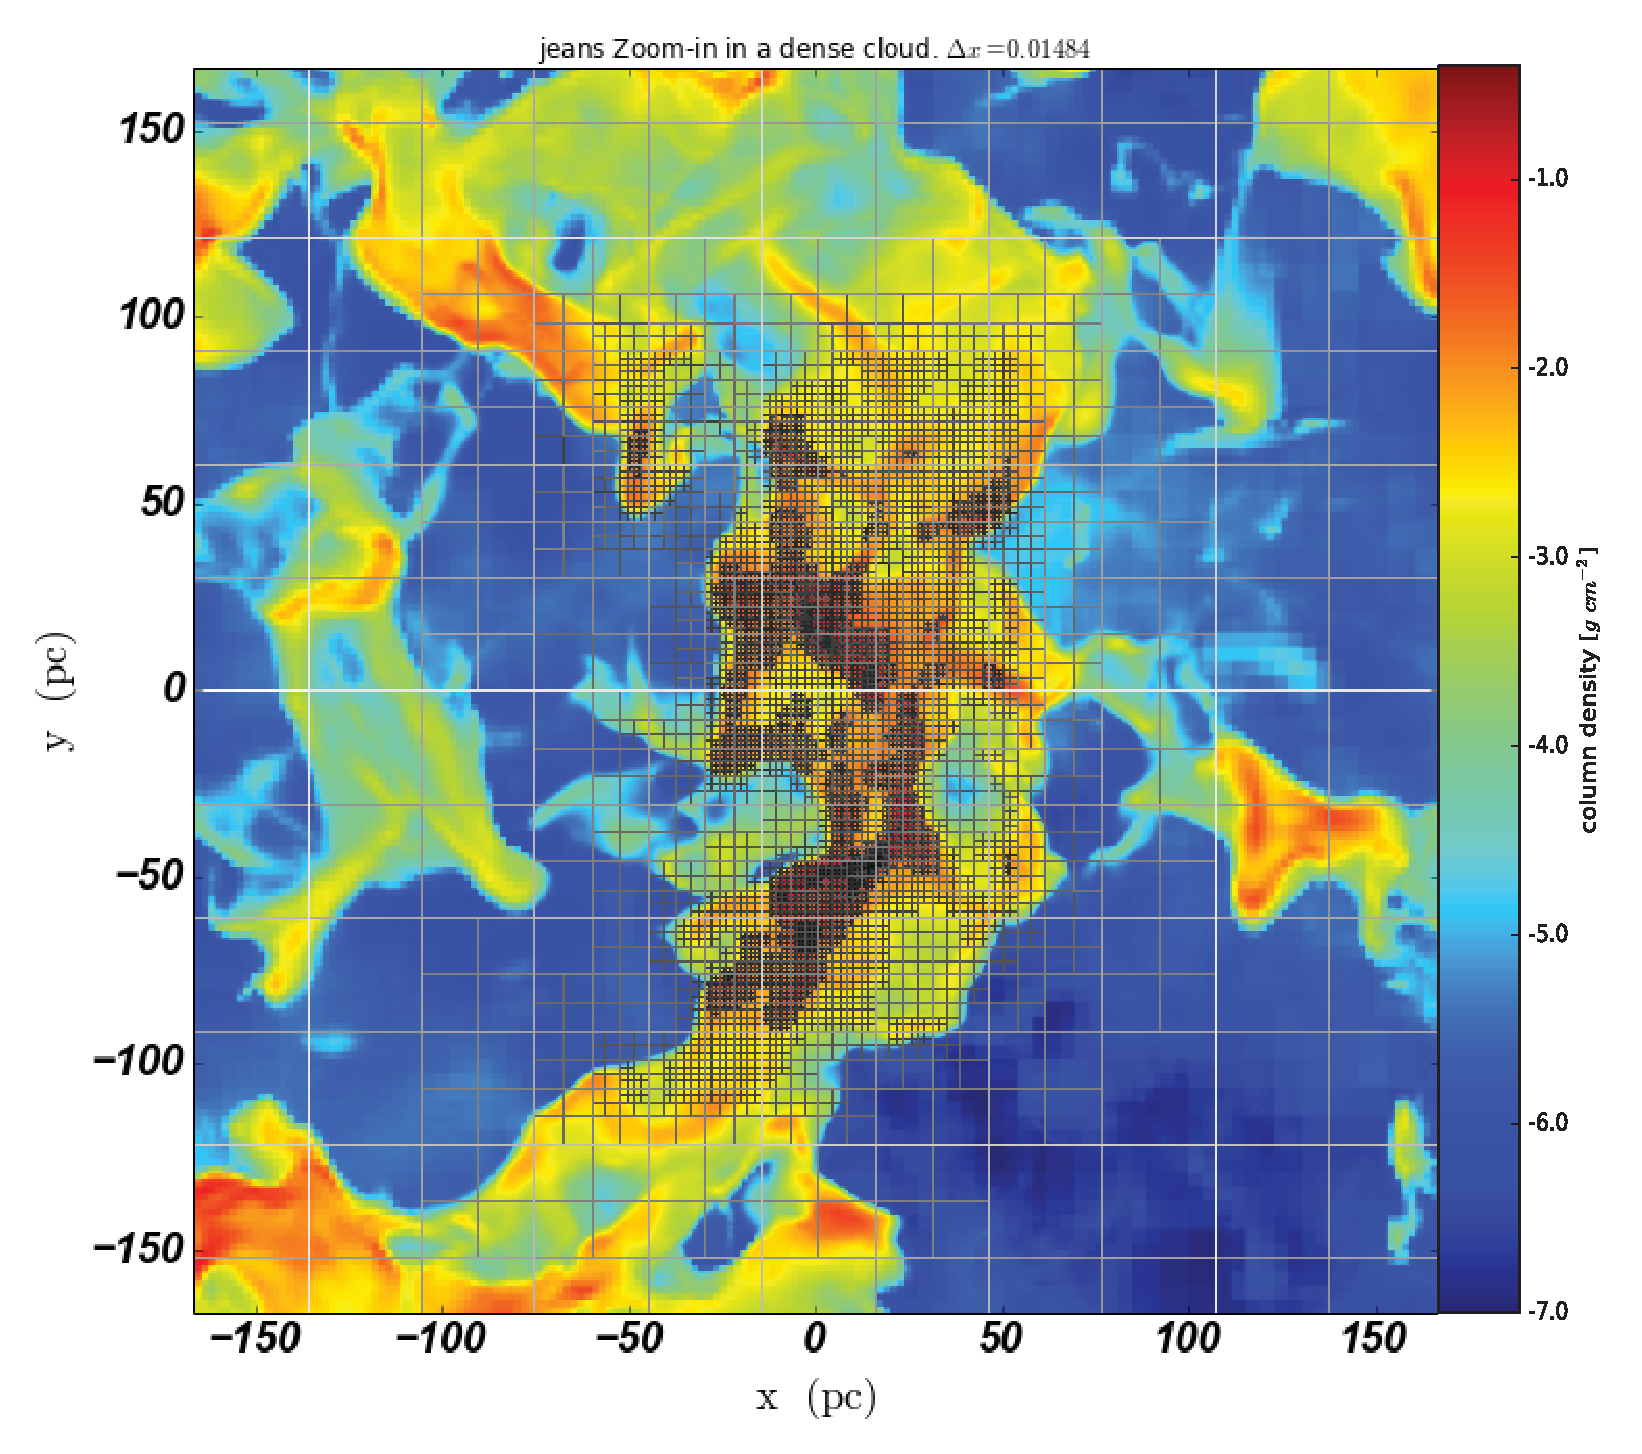
\includegraphics[scale=0.4]{Figures/DenseCloud_ZoomIn_wGrid.eps} 
	\caption{Localized zoom in refinement in a turbulent dense cloud.}	
	% Put the figure in here 
	\label{Zoom-in_cloud}
\end{figure}
	
The first set of zoom-in simulations will not include gas self-gravity in order to study the turbulent cascade down to the very small scales, the gas dynamics and formation sub-structure due to the supersonic turbulence.
Figure \ref{Zoom-in_cloud}, computed with this year's allocation, shows a column density projection of a giant molecular cloud, with the localized zoom-in conditions resolving the cloud's sub-structure on scales down to $\Delta x \approx 0.015 pc$.
	
The second set of simulations will include self-gravity to study the collapse and fragmentation of the gas and the development of the initial conditions for star formation.
	
Resolving the gas dynamics at these scales, $\Delta x \approx 10^{-2}$, compromises the accuracy of some of our approximations, such as the parametrized cooling of the gas. 
At these high densities, thermal timescales are comparable to the gas dynamical timescale and we need a more accurate description of the gas radiative cooling to accurately resolve the dynamics and fragmentation of the dense gas.
A more detailed model is limited due to the lack of live chemistry in the simulation, however we have a new parametrization for radiative  ooling from simulations including a detailed treatment of the non-equilibrium chemistry for the dust and the most important atomic and molecular species \citep{Gover&MacLow2007, Glover2010}.
The new curve accurately predicts the gas cooling rate for temperatures between $100 < T < 10 \, K$ and number densities between $10^2 < n < 10^5 \, cm^{-3}$.
		 
		
	
\section{Computational methods}
	
% Something about Flash
These set of simulations will be performed with the parallel adaptive mesh refinement (AMR) code FLASH \citep{Flash}, which is maintained by the ASC/Alliances Center for Astrophysical Thermonuclear Flashes (Flash center for computational science) at the University of Chicago.
All code units are parallelized using MPI, with excellent scalability up up to several thousands of CPU's \citep{Dubey2008, FlashPerformance}.
For these simulations we will use FLASH v4.0.1 released on February 2013.
	
% About the solvers we are using
 We will take advantage of the positive-states-preserving magnetohydrodynamics (MHD) Riemann solver developed by \citet{Bouchout2010} and implemented in FLASH v2.5 by \citet{Waagan2011} which we ported to FLASH 4.0.
The solver guarantees the positivity of density and pressure, and has proven to be highly stable over a large range of Mach numbers ($\sim 10^{-2} - 10$) and plasma $\beta$ ($\sim 10^{-2} - 10^{6}$) normally encountered in star formation simulations \citep{JoungMacLow2006,Joung2009, Hill2012}.

% Size of the Box and initial conditions & boundary conditions
The box models consist on an elongated box of size $1 \times 1 \times 40 \, kpc^{3}$, with periodic boundary conditions in the horizontal directions, and outflow in the vertical direction.
We require the box to extend to $z \pm \, 20 \, kpc$ far from the midplane to minimize the loss of matter lifted by SN explosions in a galactic fountain. 
A width of $1 \, kpc$ is necessary to be sure that the largest superbubbles in the volume do not interact with themselves.
	
% SN explosions
Supernova explosions are the main driver of turbulence in the simulation.
For each SN explosion, we add thermal energy $E_{SN} = 10^{51} \, erg$ to a sphere encompassing $100 M_{\odot}$, producing a density dependence radius of $17-100 \, pc$, chosen so that the sudden increase of temperatures does not falls below $10^{6} \, K$, avoiding radiative losses inside the sphere during the first timesteps, allowing for the development of the SN shock front. 
A fixed fraction of 3/5, of the Type II SNs are correlated in space and time to model superbubbles (SB), the vertical position of these SB correspond to the scale height of Type II SN events.
The remaining field SNs have random positions with appropriate scale heights for Type I and Type II events in the galaxy.
The SN rate is fixed and it is adjusted to the galactic SN rate.
For an accurate development of the SN explosion dynamics, a minimum resolution of $\leqslant 2 \, pc$ in the midplane is required. 
This prevents the sudden radiation of the SN energy and the mixing of hot and cold gas, in order to achieve a consistent volume filling fractions of the phases of the ISM.
	
% Galactic potential
The vertical gravitational acceleration give rise to the flat disk-like structure in the simulation and maintains the stratification of the atmosphere.
The static gravitational potential accounts for the contribution of gas, stars and dark matter in the galaxy, and is computed from a modified version of the \citet{Kuijken&Gilmore1989} potential near the midplane, $< 8 \, kpc$, and smoothly converting to the dark matter potential of the halo \citep{NFW}, as described in \citet{Hill2012}.
	
% Heating and cooling
Detailed treatment of the gas thermodynamics is required to capture the dynamics and the phases of the interstellar medium.
We implement a parametrized radiative cooling, corresponding to an optically thin plasma with solar metallicity composition \citep{Dalgarno&McCray1972, Sutherland&Dopita1993} and a diffuse heating term that accounts for the photoelectric heating \citep{Wolfire1995, Wolfire2003} of the neutral gas.
We also include a parametrized radiative cooling for the cold, $T < 100 \, K$, and dense gas, $n > 100 \, cm^{-3}$, accounting for realistic cooling timescales due to non-equilibrium chemistry, gas self shielding and dust shielding \citep{Gover&MacLow2007, Glover2010}.
In reality a detailed estimation of the gas heating and cooling requires the treatment of non-equilibrium chemistry and spatially and temporal dependence of the FUV radiation field \citep{Parravano2003}, but in the absence of a chemistry and a radiative transfer model, we resorted to the more simple parametrized cooling curves and to the power-law scaling relation relating the stellar surface density to the heating rate \citep{Joung2009}.

% About the AMR and the zoom in simulations
For the mesh refinement we plan to make use of the standard paramesh \citep{paramesh} module present in FLASH 4.01.
Due to the shape of the box and the distribution of the dense gas in the simulated volume, we implement a nested refinement structure, with the higher resolution around the midplane and lower resolution with increasing distance to the midplane.
Such nested criteria allow us to capture the evolution of the gas at altitudes in the galactic fountain, and to accurately simulate the dynamics of the dense gas and the SN explosions near the midplane.
	
For the zoom-in simulations we will use a similar methodology as one used for cosmological simulations in Flash by \citet{Sutter&Ricker2012} but we will restrain the extra mesh refinement to be localized in gravitationally unstable gas. 
We plan to define regions of size $\sim 40 - 100 \, pc^3$ for further study with our zoom-in module.
We will only refine on jeans-unstable gas, allowing us to save a factor of roughly 2.5 in volume for each zoom-in level, due to gravitational collapse and fragmentation.
We will use 13 levels of refinement, giving us a dynamic range of $\sim 8 \times 10^3$ in spatial scales and a highest resolution of $\Delta x \approx 1.5 \times 10^{-2} \, pc$, sufficient to resolve individual molecular cores within massive clumps.
We will run each realization of this model for $10 \, Myr$ to study the initial evolution of a single molecular cloud complex prior to strong influence from feedback. We will examine three different molecular cloud complexes, for a range of initial cloud masses of $10^{3} < M_{0} < 10^{5}$, in order to distinguish general characteristics of behavior from historical accidents.
	
	
% Self gravitating simulations & sink particles.
Runaway gravitational collapse quickly becomes numerically unresolved, the formation of sink particles transforms this collapsing gas into a point particle that can continue accreting gas, interacting with the gas and other sink particles, and feed back energy to the environment \cite{Bate2009, Dale2014}.
	For the calculation of the self gravitational potential we will use the existing multi-grid Poisson module in Flash.
Regions of runaway collapse will be replaced by sink particles \citep{Bate95}, once they reach the resolution limit of the simulation and satisfy a number of criteria \citep{Federrath2010}.
Our sink particle particle formalism guarantees that only gravitationally bound gas contributes in the formation of, and accretion onto the sink particle.
The behavior of the multi-grid Poisson solver with sink particle formation has been successfully tested and implemented in Flash in small scale massive star formation models \citep{Peters2010}.
Sink particles interact gravitationally with both the gas and with one another.
N-body interactions are solved using a leap-frog integrated.
	
% Radiative transfer & Wind feedback.
When a massive star forms it deposits energy into the ISM in the form of radiation, winds and end its life in a SN explosion. 
These energetic feedback is crucial for quenching the star formation efficiency in dense clouds and drive turbulence in the galaxy.
We plan to include self-consistent stellar feedback from the formed sink particles in the form of radiation, stellar winds and SN feedback.
	
For the treatment of the radiation, we have implemented and are testing the adaptive ray tracing technique developed by \citet{Wise&Abel2011}, which allows termination of rays once they reach regions of high opacity, and merging of rays if the angular distance between two sources becomes smal enough for them to be treated as one.
This approach takes advantage of the improved parallel communication routines in the new Flash version \citep{FlashPerformance}
	
For the stellar wind feedback we need to know the mass loss rate, and wind velocity at all times to cast the winds, this parameters are computed from a subset of stellar evolution tracks \citet{Ekstrom2012, Georgy2012, Georgy2013}.
	

\section{Justification of Resources}

Need to work on this a lot.


\section{Project team qualifications}

...

\section{Management}

\subsection{Summary}

The local, self-gravitating and zoom-in runs will be led by co-I Iba{\~n}ez-Mejia. 
These will be performed under the supervision of PU Mac Low, and co-I Klessen, and results will be published collaboratively.

\subsection{Local Computing Environment}

At the Museum, the PI and his group have partial access to several small clusters. 
These include a 40-processor Sunfire Ultrasparc III 900 Mhz cluster, a 256-processor cluster with 2.8 Ghz Xeons connected with Myrinet, and a 128 core (32 nodes each with two dual core processors) cluster connected with Infiniband.
Except for the Sun luster, these machines are shared with other users at the Museum including biologists doing large phylogenetic computations, and other astrophysicists. 


%\bibliographystyle{plain}
%\bibliography{MainDoc}

\bibliographystyle{aa} % style aa.bst
\bibpunct{(}{)}{;}{a}{}{,} % to follow the A&A style
% for the bibliography, at the end

%\bibliographystyle{aa} % style aa.bst

\bibliography{MainDoc}

\end{document}



